
% ------------------------------------------------------------------------------
\section{Osciladores armonicos}

\begin{definition}
    Variacion oscilatoria(periodica) de una magnitud alrededor de un punto de equilibrio.
\end{definition}

\subsection{Ejemplos}
\begin{itemize}
	\item Resortes
	\item Pendulos
	\item Ondas E.M.
\end{itemize}

\subsection{Modelos}
\begin{itemize}
	\item Suponemos muy liviano
	\item Debe estar en regimen lineal($F=k \cdot \Delta x$)
	\item Sin friccion
\end{itemize}

Por Newton:
\begin{gather}
	\nonumber F = k \cdot \Delta c = m \cdot a_x
\end{gather}

Debido al sistema de coordenadas elejido:

\begin{gather}
	\nonumber -k \cdot x = m \cdot a_x \\
	\nonumber -k \cdot x = m \cdot \ddot{x}
\end{gather}

Despejo:

\[
	\ddot{x} + \frac{k}{m} \cdot x = 0
\]

Proponemos solucion a la EDO(una manera de resolverla):

\begin{gather}
	\no x(t)=C \cdot e^{rt} \\
	\no x'(t)=rC \cdot e^{rt} \\
	\no x''(t)=r^2C \cdot e^{rt}
\end{gather}

Reemplazamos en la EDO
\begin{gather}
	\no (r^2 + \frac{k}{m})  \cdot C \cdot e^{rt} = 0 \\
	\no r^2 + \frac{k}{m} = 0 \\
	\no r = \pm i \sqrt{\frac{k}{m}}
\end{gather}

Pasamos a formula general:

\begin{gather}
	\no x(t)=C_1 \cdot e^{i\sqrt{\frac{k}{m}}t} + C_2 \cdot e^{i\sqrt{\frac{k}{m}}t} \\
	\no\text{(Oscilador armonico)}\\
	\no\text{Se definen } C_1 = \frac{A}{2}\cdot e^{i\varphi_0} 
	\no\text{ y } C_2 = \frac{A}{2}\cdot e^{-i\varphi_0}\\
\\
	\no x(t)=\frac{A}{2}\cdot e^{i\varphi_0} \cdot e^{i\sqrt{\frac{k}{m}}t} + \frac{A}{2}\cdot e^{-i\varphi_0} \cdot e^{i\sqrt{\frac{k}{m}}t}\\
	\no x(t)=\frac{A}{2}\cdot(e^{i(\sqrt{\frac{k}{m}}t + \varphi)} + e^{-i(\sqrt{\frac{k}{m}}t + \varphi)} )\\
	\text{Usamos notacion de Euler:}\\
	\no x(t) = A\cdot \cos{(\sqrt{\frac{k}{m}}t + \varphi_0)}
\end{gather}

$A$ es la amplitud, $\varphi$ es la fase(angul en cada $t$), $\varphi_0$ es el angulo inicial
($x_0=A\cdot \cos{ \varphi_0}$) y $T=\frac{2\pi}{\omega}$ es el periodo, entonces $\omega$ es la frecuencia angular. $T$ es constante, entonces $\omega$ es propiedad del sistema.

\begin{gather}
	\no x(t)= A \cdot \cos{(\omega t + \varphi_0)}\\
	\no v(t)= - A \cdot \omega \cdot \sin{(\omega t + \varphi_0)}\\
	\no v(t)= - A \cdot \omega^2 \cdot \sin{(\omega t + \varphi_0)}
\end{gather}

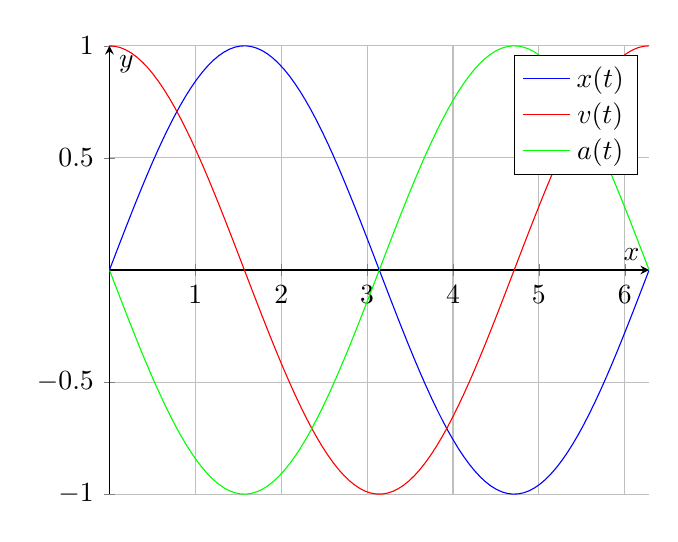
\begin{tikzpicture}
	\begin{axis}[axis lines=middle, xlabel=$x$, ylabel={$y$}, grid=major]
		\addplot[blue, domain=0:2*pi, samples=100] {sin(deg(x))};
		\addlegendentry{$x(t)$}

		\addplot[red, domain=0:2*pi, samples=100] {cos(deg(x))};
		\addlegendentry{$v(t)$}

		\addplot[green, domain=0:2*pi, samples=100] {-sin(deg(x))};
		\addlegendentry{$a(t)$}

	\end{axis}
\end{tikzpicture}

\subsection{Energia del oscilador armonico}
\begin{gather}
	\no E(\text{mecanica}) = U + K \\
	\no E = \frac{1}{2} m v^2 + \frac{1}{2} k x^2 \\
	\no E = \frac{1}{2} m A^2 \cdot \omega^2 \cdot \sin^2{(\omega t + \varphi_0)} + \frac{1}{2} k A^2 \cdot \cos^2{(\omega t + \varphi_0)}\\
	\no\text{Como } \omega=\sqrt{\frac{k}{m}} \Rightarrow k=m \omega^2
\end{gather}

Finalmente:

\[
	E=\frac{1}{2} m \omega^2 A^2 = \frac{1}{2} k A^2 
\]

Notar que es constante.


% ------------------------------------------------------------------------------

